\documentclass[a4paper,12pt]{article}

% ---------- FONT & LANGUAGE ----------
\usepackage{fontspec}
\usepackage{polyglossia}
\usepackage{caption}
\usepackage{float}

\setmainlanguage{greek}
\setotherlanguage{english}

% Γραμματοσειρές
\newfontfamily\greekfont{Times New Roman}[Script=Greek, Scale=1.0]
\newfontfamily\englishfont{Times New Roman}[Script=Latin, Scale=1.0]

% Μονοσύστημα γραμματοσειρά για ελληνικά και κώδικα
\newfontfamily\greekfonttt{Consolas}[Scale=MatchLowercase]  % Windows συχνά έχει Consolas
\newfontfamily\englishfonttt{Consolas}[Scale=MatchLowercase]

% ---------- PACKAGES ----------
\usepackage{graphicx}
\usepackage{amsmath}
\usepackage{amssymb}
\usepackage{listings}
\usepackage{xcolor}
\usepackage{geometry}
\geometry{margin=2.5cm}

% ---------- LISTINGS STYLE ----------
\lstset{
	language=C,
	basicstyle=\greekfonttt\small,
	keywordstyle=\color{blue},
	stringstyle=\color{red},
	commentstyle=\color{green!60!black},
	numbers=left,
	numberstyle=\tiny,
	stepnumber=1,
	numbersep=5pt,
	frame=single,
	breaklines=true,
	showstringspaces=false
}

% ---------- TITLE ----------
\title{Πρώτο Σετ Ασκήσεων \\ Δομές Δεδομένων 2025-2026}
\author{
	Ανδρικόπουλος Γιάννης ΑΜ: 1115519\\
	Καραπατάκης Ευθύμιος ΑΜ: 1115521\\
	Χριστοπούλου Αγγελική ΑΜ: 1115471
}
\usepackage[colorlinks=true,linkcolor=black,citecolor=black,urlcolor=black]{hyperref}
\begin{document}
	
	\maketitle
	\tableofcontents
	\newpage
	
	% ==================================================
	\section{Άσκηση 1: Ελεγκτής Έκφρασης με Στοίβα}
	
	\subsection{Εκφώνηση}
	Υλοποιήστε συνάρτηση που χρησιμοποιεί στοίβα χαρακτήρων για να ελέγξει αν μια 
	έκφραση περιέχει σωστά τοποθετημένες παρενθέσεις (), αγκύλες [] και άγκιστρα \{\}. 
	Η συνάρτηση πρέπει να επιστρέφει 1 αν η έκφραση είναι σωστή, διαφορετικά 0.
	
	\subsection{Ανάλυση}
	Για την επίλυση χρησιμοποιείται \textbf{στοίβα} (stack), η οποία ακολουθεί τη 
	λογική \textbf{LIFO} (Last In, First Out): το τελευταίο στοιχείο που εισήχθη 
	είναι το πρώτο που αφαιρείται.
	
	Η στοίβα είναι η κατάλληλη δομή για αυτό το πρόβλημα γιατί κάθε κλειστή 
	παρένθεση πρέπει να αντιστοιχεί στην πιο πρόσφατα ανοιχτή — ακριβώς η 
	συμπεριφορά που προσφέρει το LIFO.
	
	\subsubsection{Σύγκριση Υλοποιήσεων}
	Η στοίβα μπορεί να υλοποιηθεί με δύο τρόπους:
	
	\begin{itemize}
		\item \textbf{Πίνακας:} Απλή και αποδοτική υλοποίηση με σταθερό μέγεθος. 
		Η πρόσβαση γίνεται μέσω δείκτη \texttt{pos} που δείχνει στην κορυφή. 
		Μειονέκτημα: σταθερό μέγιστο μέγεθος.
		
		\item \textbf{Συνδεδεμένη Λίστα:} Δυναμικό μέγεθος χωρίς περιορισμό. 
		Κάθε κόμβος περιέχει έναν χαρακτήρα και δείκτη στον επόμενο. 
		Μειονέκτημα: επιπλέον μνήμη για δείκτες και \texttt{malloc}/\texttt{free}.
	\end{itemize}
	
	Στην παρούσα υλοποίηση επιλέχθηκε \textbf{πίνακας} για απλότητα και 
	αποδοτικότητα.
	
	\subsection{Αλγόριθμος}
	\begin{enumerate}
		\item Διατρέχουμε την έκφραση χαρακτήρα-χαρακτήρα
		\item Αν ο χαρακτήρας είναι ανοιχτή παρένθεση \texttt{(}, \texttt{[}, 
		\texttt{\{} → την εισάγουμε στη στοίβα (push)
		\item Αν είναι κλειστή παρένθεση:
		\begin{itemize}
			\item Αν η στοίβα είναι άδεια → λάθος (επιστροφή 0)
			\item Αφαιρούμε το τελευταίο στοιχείο (pop)
			\item Αν δεν αντιστοιχεί → λάθος (επιστροφή 0)
		\end{itemize}
		\item Στο τέλος: αν η στοίβα είναι άδεια → σωστό (1), αλλιώς λάθος (0)
	\end{enumerate}
	
	\subsection{Υλοποίηση}
	
	\begin{lstlisting}
		int check(char* ekfrash) {
			char stack[LENGTH];
			int pos = -1;
			int len = strlen(ekfrash);
			
			for (int i = 0; i < len; i++) {
				char ch = ekfrash[i];
				
				if (ch == '(' || ch == '[' || ch == '{') {
						stack[++pos] = ch;
					}
					else if (ch == ')' || ch == ']' || ch == '}') {
					
					if (pos == -1) return 0;
					
					char prohgoymeno = stack[pos--];
					
					if ((ch == ')' && prohgoymeno != '(') ||
					(ch == ']' && prohgoymeno != '[') ||
					(ch == '}' && prohgoymeno != '{')) {
						return 0;
					}
				}
			}
			return (pos == -1) ? 1 : 0;
		}
	\end{lstlisting}
	
	\subsection{Αποτελέσματα Εκτέλεσης}
	
	\begin{figure}[H]
		\centering
		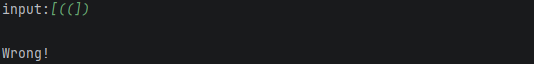
\includegraphics[width=0.7\textwidth]{askisi1Screenshot1.png}
		\caption{Εκτέλεση του προγράμματος με λάθος input}
	\end{figure}
	
	\begin{figure}[H]
		\centering
		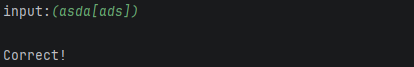
\includegraphics[width=0.7\textwidth]{askisi1Screenshot2.png}
		\caption{Εκτέλεση του προγράμματος με σωστό input}
	\end{figure}
	
	\subsection{Πολυπλοκότητα}
	\begin{itemize}
		\item \textbf{Χρονική:} $O(n)$ — κάθε χαρακτήρας επεξεργάζεται μία φορά
		\item \textbf{Χωρική:} $O(n)$ — η στοίβα στη χειρότερη περίπτωση 
		αποθηκεύει όλους τους χαρακτήρες
	\end{itemize}
	
	\subsection{Συμπεράσματα}
	Η στοίβα αποτελεί την ιδανική δομή για προβλήματα αντιστοίχισης συμβόλων, 
	καθώς η LIFO συμπεριφορά της ταιριάζει φυσικά με την εμφώλευση παρενθέσεων. 
	Η υλοποίηση με πίνακα προτιμάται για απλότητα όταν το μέγεθος εισόδου 
	είναι γνωστό, ενώ η λίστα προσφέρει ευελιξία για άγνωστο μέγεθος.
	\newpage
	
	% ==================================================
	\section{Άσκηση 2: Δυαδικό Δέντρο Αναζήτησης (BST)}
	
	\subsection{Εκφώνηση}
	Υλοποιήστε συνάρτηση με το όνομα \texttt{binaryTreeSearch} που επιχειρεί να 
	εντοπίσει μια καθορισμένη τιμή σε ένα δυαδικό δέντρο αναζήτησης με ακέραιους. 
	Η συνάρτηση δέχεται ως ορίσματα τη ρίζα του δέντρου και το κλειδί αναζήτησης. 
	Αν βρεθεί, επιστρέφει δείκτη στον κόμβο, αλλιώς \texttt{NULL}.
	
	Υλοποιήστε επίσης συναρτήσεις εισαγωγής και διαγραφής. Να γίνει έλεγχος 
	με κύριο πρόγραμμα. Να εξηγηθεί θεωρητικά η διαφορά κομβο- και 
	φυλλοπροσανατολισμένου δέντρου.
	
	\subsection{Ανάλυση}
	Το \textbf{Δυαδικό Δέντρο Αναζήτησης} (BST) είναι δομή δεδομένων όπου για 
	κάθε κόμβο ισχύει:
	\begin{itemize}
		\item Όλοι οι κόμβοι του \textbf{αριστερού} υποδέντρου έχουν τιμή 
		\textbf{μικρότερη} από τον κόμβο
		\item Όλοι οι κόμβοι του \textbf{δεξιού} υποδέντρου έχουν τιμή 
		\textbf{μεγαλύτερη} από τον κόμβο
	\end{itemize}
	
	Η ιδιότητα αυτή επιτρέπει αναζήτηση σε $O(\log n)$ για ισορροπημένο δέντρο.
	
	\subsection{Σύγκριση Υλοποιήσεων}
	
	\subsubsection{Κομβοπροσανατολισμένο Δέντρο (επιλέχθηκε)}
	Κάθε κόμβος — εσωτερικός και φύλλο — αποθηκεύει δεδομένα. Η αναζήτηση 
	μπορεί να τερματίσει σε οποιονδήποτε κόμβο.
	
	\begin{itemize}
		\item \textbf{Πλεονέκτημα:} Απλούστερη δομή, λιγότεροι κόμβοι
		\item \textbf{Μειονέκτημα:} Πιο πολύπλοκη διαγραφή (3 περιπτώσεις)
	\end{itemize}
	
	\subsubsection{Φυλλοπροσανατολισμένο Δέντρο}
	Τα δεδομένα αποθηκεύονται \textbf{μόνο στα φύλλα}. Οι εσωτερικοί κόμβοι 
	περιέχουν μόνο τιμές σύγκρισης για την καθοδήγηση της αναζήτησης.
	
	\begin{itemize}
		\item \textbf{Πλεονέκτημα:} Απλούστερη διαγραφή (αφαίρεση φύλλου)
		\item \textbf{Μειονέκτημα:} Διπλάσιοι περίπου κόμβοι, πιο περίπλοκη εισαγωγή
	\end{itemize}
	
	Αν επιλεγόταν φυλλοπροσανατολισμένο δέντρο, η δομή του κόμβου θα είχε 
	επιπλέον πεδίο για διάκριση εσωτερικού/φύλλου, και η αναζήτηση θα 
	κατέληγε πάντα σε φύλλο.
	
	\subsection{Βασικές Συναρτήσεις}
	
	\subsubsection{Αναζήτηση}
	Αναδρομική συνάρτηση που εκμεταλλεύεται την ιδιότητα BST:
	
	\begin{lstlisting}
		struct Node* binaryTreeSearch(struct Node* node, int target) {
			if (node == NULL)       return NULL;
			if (node->data == target) return node;
			
			if (target < node->data)
			return binaryTreeSearch(node->left, target);
			else
			return binaryTreeSearch(node->right, target);
		}
	\end{lstlisting}
	
	\subsubsection{Εισαγωγή}
	Βρίσκει αναδρομικά την κατάλληλη κενή θέση και τοποθετεί νέο κόμβο:
	
	\begin{lstlisting}
		struct Node* insert(struct Node* node, int value) {
			if (node == NULL) return createNode(value);
			
			if (value < node->data)
			node->left = insert(node->left, value);
			else if (value > node->data)
			node->right = insert(node->right, value);
			else
			printf("The value %d is already in the tree!\n", value);
			
			return node;
		}
	\end{lstlisting}
	
	\subsubsection{Διαγραφή}
	Η διαγραφή αντιμετωπίζει τρεις περιπτώσεις:
	
	\begin{enumerate}
		\item \textbf{Φύλλο (0 παιδιά):} Απελευθερώνεται η μνήμη, επιστρέφεται \texttt{NULL}
		\item \textbf{Ένα παιδί:} Ο γονέας συνδέεται απευθείας με το παιδί
		\item \textbf{Δύο παιδιά:} Αντικαθίσταται η τιμή με τον \textit{inorder successor} 
		(ελάχιστο του δεξιού υποδέντρου) και διαγράφεται ο successor
	\end{enumerate}
	
	\begin{lstlisting}
		struct Node* deleteNode(struct Node* node, int value) {
			if (node == NULL) return NULL;
			
			if (value < node->data)
			node->left = deleteNode(node->left, value);
			else if (value > node->data)
			node->right = deleteNode(node->right, value);
			else {
				if (node->left == NULL && node->right == NULL) {
					free(node); return NULL;
				}
				else if (node->left == NULL) {
					struct Node* temp = node->right;
					free(node); return temp;
				}
				else if (node->right == NULL) {
					struct Node* temp = node->left;
					free(node); return temp;
				}
				else {
					struct Node* successor = findMin(node->right);
					node->data = successor->data;
					node->right = deleteNode(node->right, successor->data);
				}
			}
			return node;
		}
	\end{lstlisting}
	
	\subsection{Δεδομένα Εισόδου}
	Το δέντρο κατασκευάζεται από το αρχείο \texttt{numbers2.txt}:
	
	\begin{center}
		10, 20, 30, 40, 50, 60
	\end{center}
	
	Οι τιμές εισάγονται σειριακά. Επειδή είναι ήδη ταξινομημένες, το δέντρο 
	εκφυλίζεται σε \textbf{λίστα} (skewed tree) με ύψος 5, που αποτελεί τη 
	\textbf{χειρότερη περίπτωση} για BST:
	
	\begin{center}
		$10 \rightarrow 20 \rightarrow 30 \rightarrow 40 \rightarrow 50 \rightarrow 60$
	\end{center}
	
	\subsection{Αποτελέσματα Εκτέλεσης}
	
	\begin{figure}[H]
		\centering
		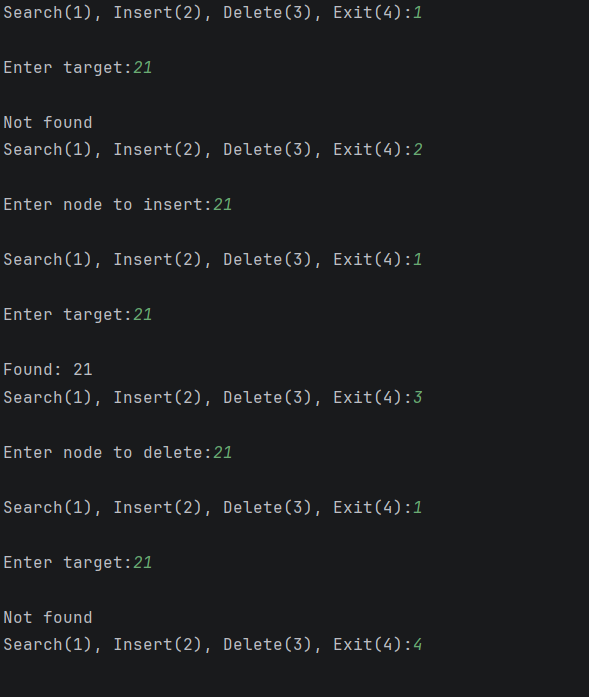
\includegraphics[height=7cm, keepaspectratio]{askisi2Screenshot1.png}
		\caption{Εκτέλεση λειτουργιών στο δυαδικό δέντρο}
	\end{figure}
	
	\subsection{Πολυπλοκότητα}
	\begin{itemize}
		\item \textbf{Μέση περίπτωση:} $O(\log n)$ για ισορροπημένο δέντρο
		\item \textbf{Χειρότερη περίπτωση:} $O(n)$ για εκφυλισμένο δέντρο 
		(όπως στα δεδομένα εισόδου μας)
	\end{itemize}
	
	\subsection{Συμπεράσματα}
	Το BST προσφέρει αποδοτική διαχείριση δεδομένων, αλλά η απόδοσή του 
	εξαρτάται από την ισορροπία του. Η επιλογή κομβοπροσανατολισμένης 
	υλοποίησης μειώνει τον αριθμό κόμβων, ενώ η διαγραφή με inorder successor 
	διατηρεί την ιδιότητα BST και στις πιο σύνθετες περιπτώσεις.
	\newpage
	
	% ==================================================
	\section{Άσκηση 3: Διαπεράσεις Δυαδικού Δέντρου}
	
	\subsection{Εκφώνηση}
	(i) Υλοποιήστε συνάρτηση \texttt{levelOrder} για τη διέλευση δυαδικού δέντρου 
	κατά επίπεδα χρησιμοποιώντας ουρά.
	
	(ii) Υλοποιήστε επίσης τις διαπεράσεις προδιάταξης (preorder) και μεταδιάταξης 
	(postorder). Να γίνει έλεγχος με κύριο πρόγραμμα.
	
	\subsection{Ανάλυση}
	Η διαπέραση ενός δυαδικού δέντρου είναι η διαδικασία επίσκεψης όλων των κόμβων 
	με συγκεκριμένη σειρά. Υπάρχουν δύο βασικές κατηγορίες:
	
	\begin{itemize}
		\item \textbf{DFS (Depth-First Search):} Αναδρομικές διαπεράσεις που 
		ακολουθούν ένα μονοπάτι μέχρι το φύλλο πριν επιστρέψουν. 
		Περιλαμβάνει preorder, inorder, postorder.
		\item \textbf{BFS (Breadth-First Search):} Μη αναδρομική διαπέραση κατά 
		επίπεδα (level order) που χρησιμοποιεί \textbf{ουρά}.
	\end{itemize}
	
	\subsection{Διαπέραση κατά Επίπεδα (Level Order / BFS)}
	Η διαπέραση αυτή επισκέπτεται τους κόμβους επίπεδο-επίπεδο, από αριστερά 
	προς τα δεξιά. \textbf{Δεν είναι αναδρομική} — χρησιμοποιεί ουρά (FIFO) 
	για να εξασφαλίσει τη σωστή σειρά επεξεργασίας.
	
	\subsubsection{Αλγόριθμος}
	\begin{enumerate}
		\item Εισάγουμε τη ρίζα στην ουρά
		\item Όσο η ουρά δεν είναι άδεια:
		\begin{itemize}
			\item Αφαιρούμε τον πρώτο κόμβο (dequeue)
			\item Εκτυπώνουμε την τιμή του
			\item Αν έχει αριστερό παιδί → το εισάγουμε στην ουρά (enqueue)
			\item Αν έχει δεξί παιδί → το εισάγουμε στην ουρά (enqueue)
		\end{itemize}
	\end{enumerate}
	
	\subsubsection{Υλοποίηση}
	\begin{lstlisting}
		void levelOrder(struct Node* n) {
			if (n == NULL) return;
			
			struct Queue q;
			initializeQueue(&q);
			add_to_queue(&q, n);        
			
			while (!isEmpty(&q)) {
				struct Node* current = remove_from_queue(&q);
				printf("%d ", current->data);
				
				if (current->left != NULL)
				add_to_queue(&q, current->left);
				if (current->right != NULL)
				add_to_queue(&q, current->right);
			}
		}
	\end{lstlisting}
	
	\subsection{Προδιάταξη (Preorder)}
	Σειρά επίσκεψης: \textbf{Ρίζα → Αριστερό → Δεξί}
	
	Χρήσιμη για: αντιγραφή δέντρου, παραγωγή prefix έκφρασης.
	
	\begin{lstlisting}
		void preorder(struct Node* n) {
			if (n == NULL) return;
			printf("%d ", n->data);   /* 1. Ριζα */
			preorder(n->left);        /* 2. Αριστερα */
			preorder(n->right);       /* 3. Δεξια */
		}
	\end{lstlisting}
	
	\subsection{Μεταδιάταξη (Postorder)}
	Σειρά επίσκεψης: \textbf{Αριστερό → Δεξί → Ρίζα}
	
	Χρήσιμη για: διαγραφή δέντρου, παραγωγή postfix έκφρασης.
	
	\begin{lstlisting}
		void postorder(struct Node* n) {
			if (n == NULL) return;
			postorder(n->left);       /* 1. Αριστερα */
			postorder(n->right);      /* 2. Δεξια */
			printf("%d ", n->data);   /* 3. Ριζα */
		}
	\end{lstlisting}
	
	\subsection{Υλοποίηση Ουράς}
	Η ουρά υλοποιείται με \textbf{πίνακα σταθερού μεγέθους} (γραμμική ουρά).
	
	\begin{lstlisting}
		void add_to_queue(struct Queue *q, struct Node* n) {
			if (isFull(q)) { printf("Queue is full\n"); return; }
			q->rear++;
			q->items[q->rear] = n;
		}
		
		struct Node* remove_from_queue(struct Queue *q) {
			if (isEmpty(q)) { printf("Queue is empty\n"); return NULL; }
			q->front++;
			return q->items[q->front];
		}
	\end{lstlisting}
	
	\subsubsection{Γραμμική vs Κυκλική Ουρά}
	Η παρούσα υλοποίηση είναι \textbf{γραμμική}: μόλις ο \texttt{rear} φτάσει 
	στο τέλος του πίνακα, η ουρά θεωρείται γεμάτη ακόμα κι αν υπάρχουν κενές 
	θέσεις στην αρχή.
	
	Στο level order traversal αυτό δεν αποτελεί πρόβλημα, καθώς κάθε κόμβος 
	εισάγεται \textbf{ακριβώς μία φορά}. Για γενικότερη χρήση θα προτιμούσαμε 
	\textbf{κυκλική ουρά} με:
	
	\begin{lstlisting}
		q->rear = (q->rear + 1) % BUFFER;
	\end{lstlisting}
	
	\subsection{Αποτελέσματα Εκτέλεσης}
	Το δέντρο κατασκευάζεται από το αρχείο \texttt{numbers3.txt}:
	
	\begin{center}
		50, 25, 75, 10, 30, 60, 90, 5, 15, 27, 35, 55, 65, 85, 95, 1, 8, 12, 18, 28
	\end{center}
	
	\begin{figure}[H]
		\centering
		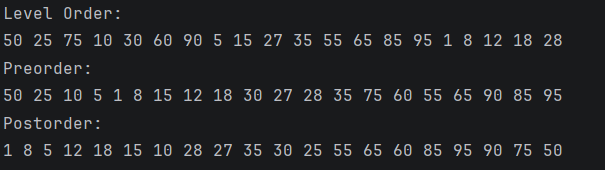
\includegraphics[width=0.7\textwidth]{askisi3Screenshot1.png}
		\caption{Αποτελέσματα διαπεράσεων του δέντρου}
	\end{figure}
	
	\subsection{Πολυπλοκότητα}
	Όλες οι διαπεράσεις επισκέπτονται κάθε κόμβο \textbf{ακριβώς μία φορά}:
	
	\begin{itemize}
		\item \textbf{Χρονική πολυπλοκότητα:} $O(n)$ για όλες τις διαπεράσεις
		\item \textbf{Χωρική πολυπλοκότητα:} $O(n)$ — λόγω ουράς (level order) 
		ή στοίβας αναδρομής (preorder/postorder). Στη χειρότερη περίπτωση η 
		στοίβα αναδρομής φτάνει βάθος $O(h)$, όπου $h$ το ύψος του δέντρου.
	\end{itemize}
	
	\subsection{Συμπεράσματα}
	Οι διαπεράσεις αποτελούν θεμελιώδη εργαλεία επεξεργασίας δέντρων. Η επιλογή 
	μεθόδου εξαρτάται από το πρόβλημα: το level order είναι ιδανικό για 
	επεξεργασία επιπέδων, το preorder για αντιγραφή/σειριοποίηση, και το 
	postorder για διαγραφή ή υπολογισμό postfix εκφράσεων.
	\newpage
	
	% ==================================================
	\section{Άσκηση 4: Ύψος και Βάθος Δυαδικού Δέντρου}
	
	\subsection{Εκφώνηση}
	Αξιοποιώντας τις διαπεράσεις του προηγούμενου ερωτήματος, υλοποιήστε:
	\begin{itemize}
		\item Συνάρτηση υπολογισμού \textbf{ύψους} δυαδικού δέντρου
		\item Συνάρτηση υπολογισμού και εκτύπωσης \textbf{βάθους} κάθε κόμβου
	\end{itemize}
	
	\subsection{Ανάλυση}
	
	\subsubsection{Ύψος Δέντρου}
	Το \textbf{ύψος} ενός δυαδικού δέντρου ορίζεται ως ο αριθμός \textbf{ακμών} 
	στο μακρύτερο μονοπάτι από τη ρίζα ως ένα φύλλο.
	
	Σύμβαση:
	\begin{itemize}
		\item Κενό δέντρο (\texttt{NULL}): ύψος $= -1$
		\item Φύλλο (κόμβος χωρίς παιδιά): ύψος $= 0$
	\end{itemize}
	
	\subsubsection{Βάθος Κόμβου}
	Το \textbf{βάθος} ενός κόμβου είναι ο αριθμός \textbf{ακμών} από τη ρίζα 
	ως τον κόμβο.
	
	Σύμβαση:
	\begin{itemize}
		\item Ρίζα: βάθος $= 0$
		\item Παιδιά ρίζας: βάθος $= 1$
		\item Εγγόνια ρίζας: βάθος $= 2$, κ.ο.κ.
	\end{itemize}
	
	\subsubsection{Σχέση Ύψους και Βάθους}
	Για οποιονδήποτε κόμβο $v$ σε \textbf{πλήρως ισορροπημένο} δέντρο ισχύει:
	$$\text{ύψος}(v) + \text{βάθος}(v) = \text{ύψος δέντρου}$$
	
	\subsection{Υλοποίηση}
	
	\subsubsection{Ύψος Δέντρου}
	Η συνάρτηση υπολογίζει αναδρομικά το ύψος από τα φύλλα προς τη ρίζα 
	(bottom-up), επιστρέφοντας σε κάθε βήμα $1 + \max(\text{ύψος\_αριστερά}, 
	\text{ύψος\_δεξιά})$:
	
	\begin{lstlisting}
		int treeHeight(struct Node* n) {
			if (n == NULL) return -1;
			
			int left  = treeHeight(n->left);
			int right = treeHeight(n->right);
			
			return 1 + (left > right ? left : right);
		}
	\end{lstlisting}
	
	Παράδειγμα υπολογισμού για τα δεδομένα μας:
	\begin{center}
		\begin{tabular}{|c|c|}
			\hline
			\textbf{Κόμβος} & \textbf{Ύψος} \\
			\hline
			1 (φύλλο) & 0 \\
			5          & 1 \\
			10         & 2 \\
			25         & 3 \\
			50 (ρίζα)  & 4 \\
			\hline
		\end{tabular}
	\end{center}
	
	\subsubsection{Βάθος Κόμβων}
	Χρησιμοποιεί preorder διάσχιση (top-down): ξεκινά από τη ρίζα με βάθος 0 
	και αυξάνει κατά 1 σε κάθε επίπεδο:
	
	\begin{lstlisting}
		void treeDepth(struct Node* n, int depth) {
			if (n == NULL) return;
			
			printf("Node: %2d,  Depth: %d\n", n->data, depth);
			
			treeDepth(n->left,  depth + 1);
			treeDepth(n->right, depth + 1);
		}
	\end{lstlisting}
	
	\subsection{Δεδομένα Εισόδου}
	Το δέντρο κατασκευάζεται από το αρχείο \texttt{numbers4.txt}:
	
	\begin{center}
		50, 25, 75, 10, 30, 60, 90, 5, 15, 27, 35, 55, 65, 85, 95, 1, 8, 12, 18, 28
	\end{center}
	
	Το δέντρο είναι \textbf{πλήρως ισορροπημένο} (perfect binary tree στα 
	επίπεδα 0--3, με επιπλέον κόμβους στο επίπεδο 4), οπότε το αναμενόμενο 
	ύψος είναι \textbf{4}. Το μακρύτερο μονοπάτι είναι π.χ.:
	$$50 \rightarrow 25 \rightarrow 10 \rightarrow 5 \rightarrow 1$$
	\subsection{Αποτελέσματα Εκτέλεσης}
	
	\begin{figure}[H]
		\centering
		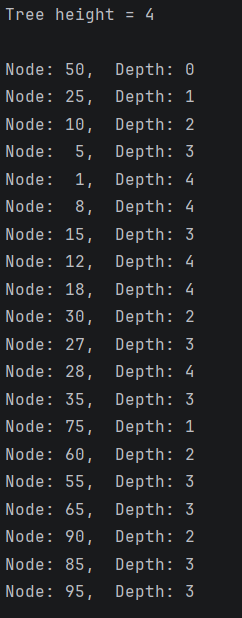
\includegraphics[height=15cm, keepaspectratio]{askisi4Screenshot1.png}
		\caption{Ύψος δέντρου και βάθος κόμβων}
	\end{figure}
	
	Αναμενόμενη έξοδος (μερική):
	\begin{lstlisting}
		Tree height = 4
		
		Node: 50,  Depth: 0
		Node: 25,  Depth: 1
		Node: 10,  Depth: 2
		Node:  5,  Depth: 3
		Node:  1,  Depth: 4
		Node:  8,  Depth: 4
		Node: 15,  Depth: 3
		...
	\end{lstlisting}
	
	\subsection{Πολυπλοκότητα}
	\begin{itemize}
		\item \textbf{Χρονική:} $O(n)$ — κάθε κόμβος επισκέπτεται ακριβώς μία φορά
		\item \textbf{Χωρική:} $O(h)$ — λόγω στοίβας αναδρομής, όπου $h$ το ύψος 
		του δέντρου. Στη χειρότερη περίπτωση (εκφυλισμένο δέντρο) $h = n$, 
		άρα $O(n)$.
	\end{itemize}
	
	\subsection{Συμπεράσματα}
	Ο υπολογισμός ύψους και βάθους αξιοποιεί τις αναδρομικές τεχνικές διαπέρασης 
	της Άσκησης 3. Το ύψος υπολογίζεται \textbf{bottom-up} (από φύλλα προς ρίζα), 
	ενώ το βάθος \textbf{top-down} (από ρίζα προς φύλλα). Οι συναρτήσεις αυτές 
	αποτελούν τη βάση για πιο σύνθετες λειτουργίες όπως έλεγχος ισορροπίας 
	δέντρου και AVL rotations.
	\newpage
	
	% ==================================================
	\section{Άσκηση 5: Ανάπλαση Δυαδικού Δέντρου από Διαπεράσεις}
	
	\subsection{Εκφώνηση}
	Δίνεται δυαδικό δέντρο με μοναδικούς χαρακτήρες. Να εξηγηθεί και να 
	υλοποιηθεί η ανάπλαση του δέντρου όταν δίνονται:
	\begin{itemize}
		\item Ενδοδιαπέραση (Inorder) + Μεταδιαπέραση (Postorder)
		\item Ενδοδιαπέραση (Inorder) + Προδιαπέραση (Preorder)
	\end{itemize}
	Να επιβεβαιωθεί το αποτέλεσμα καλώντας μία από τις συναρτήσεις διαπέρασης 
	της Άσκησης 3.
	
	\subsection{Θεωρητική Ανάλυση}
	
	Η ανακατασκευή δυαδικού δέντρου είναι δυνατή μόνο με \textbf{συγκεκριμένους 
		συνδυασμούς} διαπεράσεων, υπό την προϋπόθεση ότι οι χαρακτήρες είναι 
	\textbf{μοναδικοί}.
	
	\begin{center}
		\begin{tabular}{|l|c|}
			\hline
			\textbf{Συνδυασμός} & \textbf{Μοναδική ανακατασκευή;} \\
			\hline
			Inorder + Preorder  & \checkmark Ναι \\
			Inorder + Postorder & \checkmark Ναι \\
			Preorder + Postorder (μόνο) & \texttimes{} Όχι πάντα \\
			\hline
		\end{tabular}
	\end{center}
	
	Το \textbf{inorder είναι απαραίτητο}: είναι η μόνη διαπέραση που χωρίζει 
	καθαρά το αριστερό από το δεξί υποδέντρο. Χωρίς αυτό δεν μπορούμε να 
	προσδιορίσουμε μοναδικά τη δομή.
	
	\subsubsection{Λογική Ανακατασκευής}
	Και στις δύο περιπτώσεις η ιδέα είναι ίδια:
	\begin{enumerate}
		\item \textbf{Βρίσκουμε τη ρίζα} από το preorder (πρώτο στοιχείο) 
		ή postorder (τελευταίο στοιχείο)
		\item \textbf{Εντοπίζουμε τη ρίζα στο inorder} — ό,τι είναι αριστερά 
		της ανήκει στο αριστερό υποδέντρο, ό,τι δεξιά στο δεξί
		\item \textbf{Εφαρμόζουμε αναδρομικά} για κάθε υποδέντρο
	\end{enumerate}
	
	\subsubsection{Παράδειγμα Χειροκίνητης Ανακατασκευής}
	Δεδομένα:
	\begin{itemize}
		\item Inorder:   \texttt{D B E A F C}
		\item Preorder:  \texttt{A B D E C F}
		\item Postorder: \texttt{D E B F C A}
	\end{itemize}
	
	Από το preorder: ρίζα = \texttt{A}. 
	Στο inorder η \texttt{A} βρίσκεται στη θέση 3:
	$$\underbrace{D\ B\ E}_{\text{αριστερό}}\ |\ A\ |\ \underbrace{F\ C}_{\text{δεξί}}$$
	
	Εφαρμόζουμε αναδρομικά και παίρνουμε:
	
	\begin{center}
		\begin{tabular}{ccccc}
			& & A & & \\
			& $\swarrow$ & & $\searrow$ & \\
			& B & & C & \\
			$\swarrow$ & $\searrow$ & & $\swarrow$ & \\
			D & & E & F & \\
		\end{tabular}
	\end{center}
	
	\subsection{Αλγόριθμος Ανακατασκευής από Preorder + Inorder}
	
	\begin{enumerate}
		\item Το \texttt{preorder[preIndex]} είναι η ρίζα του τρέχοντος υποδέντρου
		\item Εντοπίζουμε τη ρίζα στο \texttt{inorder[left..right]}
		\item Αναδρομή \textbf{πρώτα αριστερά}, μετά δεξιά 
		(ακολουθεί τη σειρά του preorder)
	\end{enumerate}
	
	\begin{lstlisting}
		struct Node* buildTreePreRecursive(char inorder[], char preorder[],
		int *preIndex, int left, int right) {
			if (left > right) return NULL;
			
			char rootVal = preorder[*preIndex];
			(*preIndex)++;
			struct Node* root = createNode(rootVal);
			
			int index = search(inorder, rootVal, left, right);
			
			root->left  = buildTreePreRecursive(inorder, preorder,
			preIndex, left, index - 1);
			root->right = buildTreePreRecursive(inorder, preorder,
			preIndex, index + 1, right);
			return root;
		}
	\end{lstlisting}
	
	\subsection{Αλγόριθμος Ανακατασκευής από Postorder + Inorder}
	
	\begin{enumerate}
		\item Το \texttt{postorder[postIndex]} είναι η ρίζα (διαβάζουμε \textbf{ανάποδα})
		\item Εντοπίζουμε τη ρίζα στο \texttt{inorder[left..right]}
		\item Αναδρομή \textbf{πρώτα δεξιά}, μετά αριστερά — κρίσιμο! 
		(λόγω ανάποδης ανάγνωσης του postorder)
	\end{enumerate}
	
	\begin{lstlisting}
		struct Node* buildTreePostRecursive(char inorder[], char postorder[],
		int *postIndex, int left, int right) {
			if (left > right) return NULL;
			
			char rootVal = postorder[*postIndex];
			(*postIndex)--;
			struct Node* root = createNode(rootVal);
			
			int index = search(inorder, rootVal, left, right);
			
			root->right = buildTreePostRecursive(inorder, postorder,
			postIndex, index + 1, right);
			root->left  = buildTreePostRecursive(inorder, postorder,
			postIndex, left, index - 1);
			return root;
		}
	\end{lstlisting}
	
	\subsection{Επιβεβαίωση Ορθότητας}
	Για επιβεβαίωση εφαρμόζουμε και τις τρεις διαπεράσεις (από Άσκηση 4) 
	στο ανακατασκευασμένο δέντρο και συγκρίνουμε με τα αρχικά δεδομένα:
	
	\begin{lstlisting}
		printf("Inorder: ");
		inorderPrint(preRoot);
		
		printf("Preorder: ");
		preorderPrint(preRoot);
		
		printf("Postorder: ");
		postorderPrint(preRoot);
	\end{lstlisting}
	
	\subsection{Δεδομένα Ελέγχου και Αποτελέσματα}
	
	\begin{center}
		\begin{tabular}{|l|l|}
			\hline
			\textbf{Διαπέραση} & \textbf{Τιμή} \\
			\hline
			Inorder   & D B E A F C \\
			Preorder  & A B D E C F \\
			Postorder & D E B F C A \\
			\hline
		\end{tabular}
	\end{center}
	
	\begin{figure}[H]
		\centering
		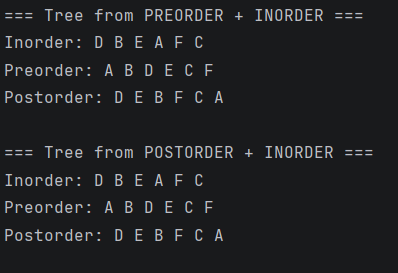
\includegraphics[width=0.7\textwidth]{askisi5Screenshot1.png}
		\caption{Επιβεβαίωση ανακατασκευασμένου δέντρου}
	\end{figure}
	
	Και τα δύο δέντρα (από preorder και postorder) παράγουν το ίδιο inorder 
	\texttt{D B E A F C}, επιβεβαιώνοντας την ορθότητα της ανακατασκευής.
	
	\subsection{Πολυπλοκότητα}
	\begin{itemize}
		\item \textbf{Χρονική:} $O(n^2)$ — για κάθε κόμβο η \texttt{search} 
		διατρέχει γραμμικά το inorder. Με χρήση \texttt{hash map} για 
		την αναζήτηση θα μειωνόταν σε $O(n)$.
		\item \textbf{Χωρική:} $O(n)$ — για την αποθήκευση του δέντρου 
		και τη στοίβα αναδρομής βάθους $O(h)$
	\end{itemize}
	
	\subsection{Συμπεράσματα}
	Η ανακατασκευή δυαδικού δέντρου από δύο διαπεράσεις είναι εφικτή μόνο 
	όταν η μία είναι το \textbf{inorder}, καθώς αυτό παρέχει τη μοναδική 
	πληροφορία διαχωρισμού αριστερού/δεξιού υποδέντρου. Η τεχνική αυτή 
	χρησιμοποιείται σε parsing, compilers και προβλήματα σειριοποίησης δέντρων.
	
\end{document}